\frame{
	\frametitle{Second Indexing Theorem}

	\begin{theorem}
		\[
			\abs{\beta_i - \beta_j} \le 1 \qquad \forall \; i, j \in \cbracket{0, \dotsc, length(\beta)-1}
		\]
	\end{theorem}

	\pause

	\begin{example}
		\begin{itemize}
			\item $\alpha = hvvhhvvvhvvhhvhhvvvvhvvvh \qquad \beta = (2, 0, 3, 2, 0, 1, 2, 4, 3)$
			\item $\alpha = hvvvvhvvvvhvhvvvhvvvvvvvh \qquad \beta = (4, 4, 1, 3, 7)$
			\item $\alpha = hvvvvhvvvvhvvvhvvvvhvvvvh \qquad \beta = (4, 4, 3, 4, 4)$
		\end{itemize}
	\end{example}
}

\frame{
	\frametitle{Second Indexing Theorem}

	\begin{theorem}
		\[
			\abs{\beta_i - \beta_j} \le 1 \qquad \forall \; i, j \in \cbracket{0, \dotsc, length(\beta)-1}
		\]
	\end{theorem}

	\begin{example}
		\begin{itemize}
			\item \sout{$\alpha = hvvhhvvvhvvhhvhhvvvvhvvvh \qquad \beta = (2, 0, 3, 2, 0, 1, 2, 4, 3)$}
			\item \sout{$\alpha = hvvvvhvvvvhvhvvvhvvvvvvvh \qquad \beta = (4, 4, 1, 3, 7)$}
			\item $\alpha = hvvvvhvvvvhvvvhvvvvhvvvvh \qquad \beta = (4, 4, 3, 4, 4)$
		\end{itemize}
	\end{example}
}

\frame{
	\frametitle{Windowing}
	\begin{figure}
    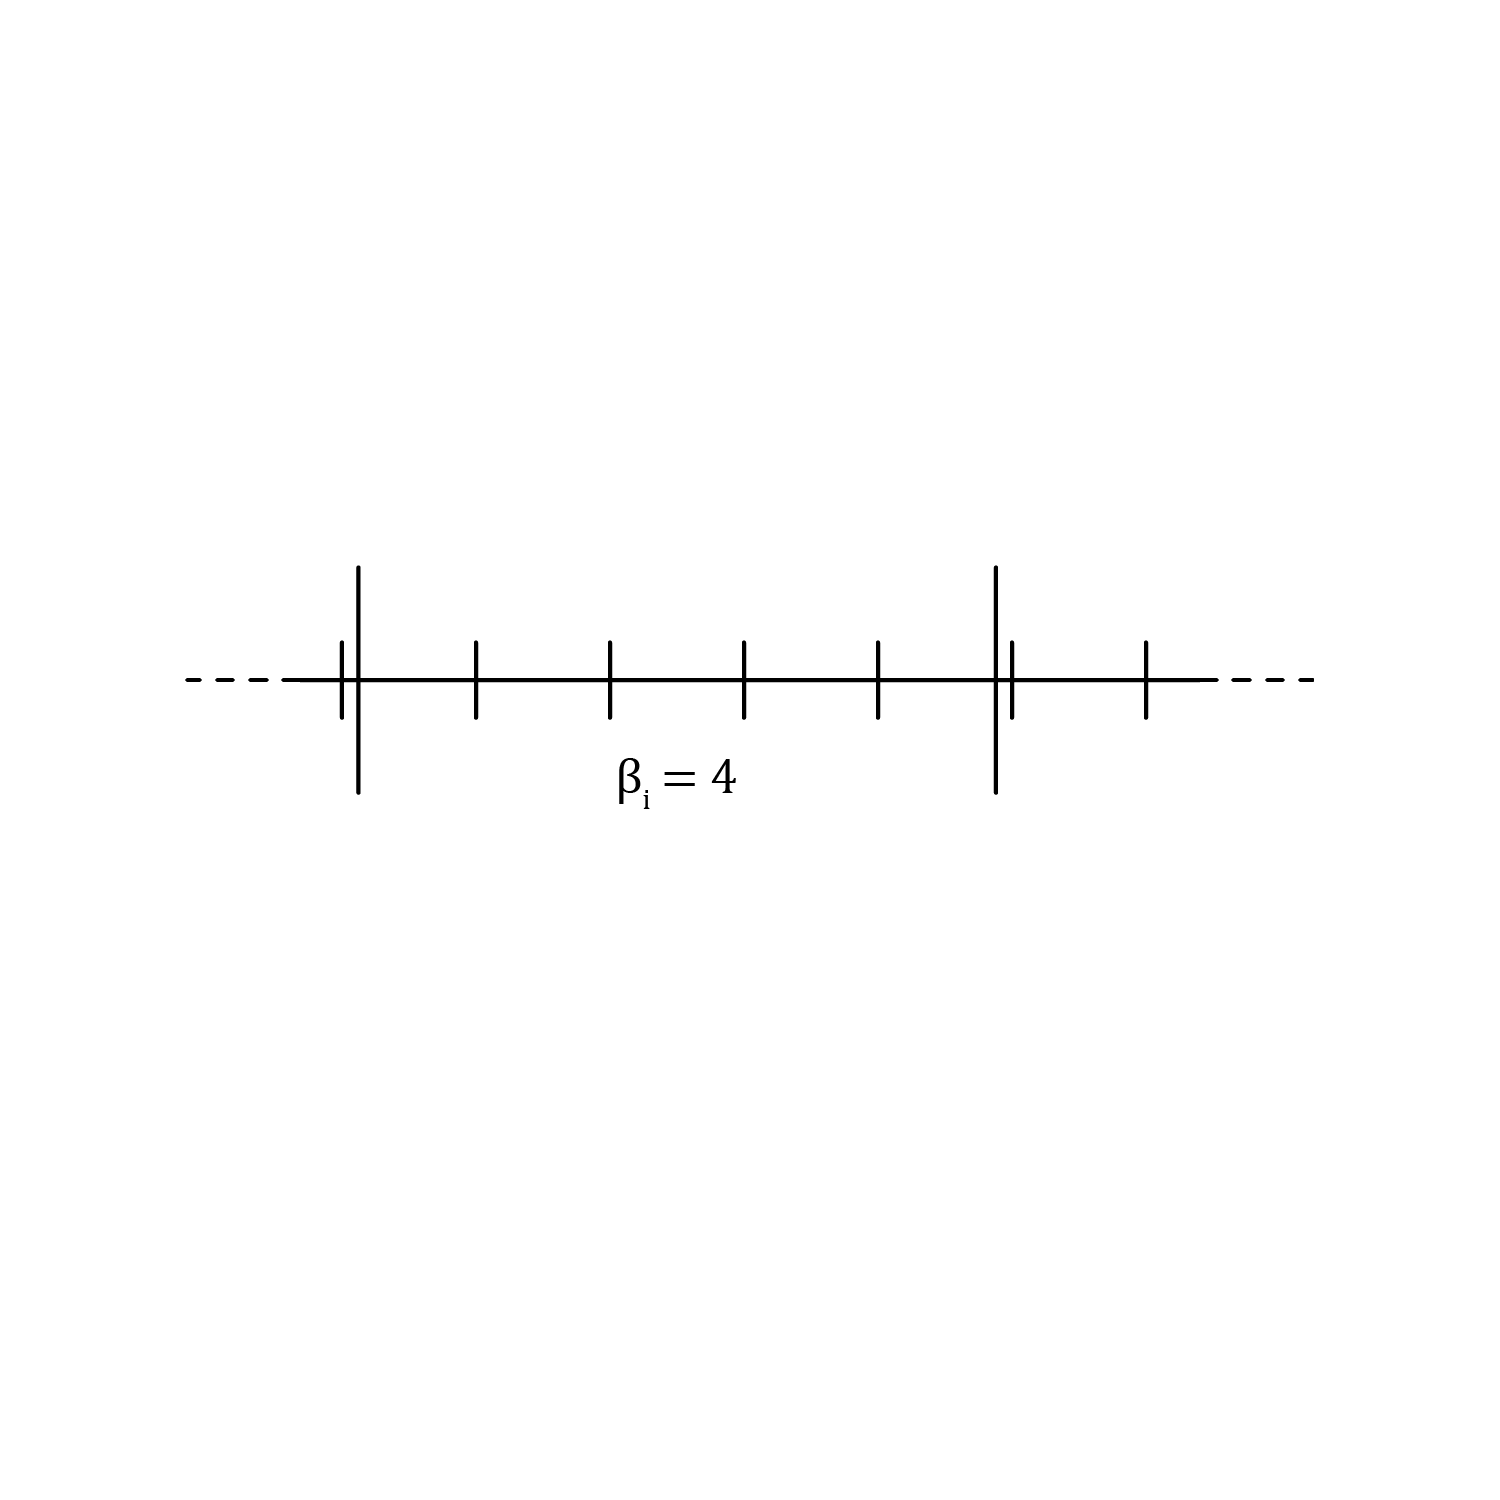
\includegraphics[width=3in]{sliding-window_1}
  \end{figure}
}

\frame{
	\frametitle{Windowing}
	\begin{figure}
    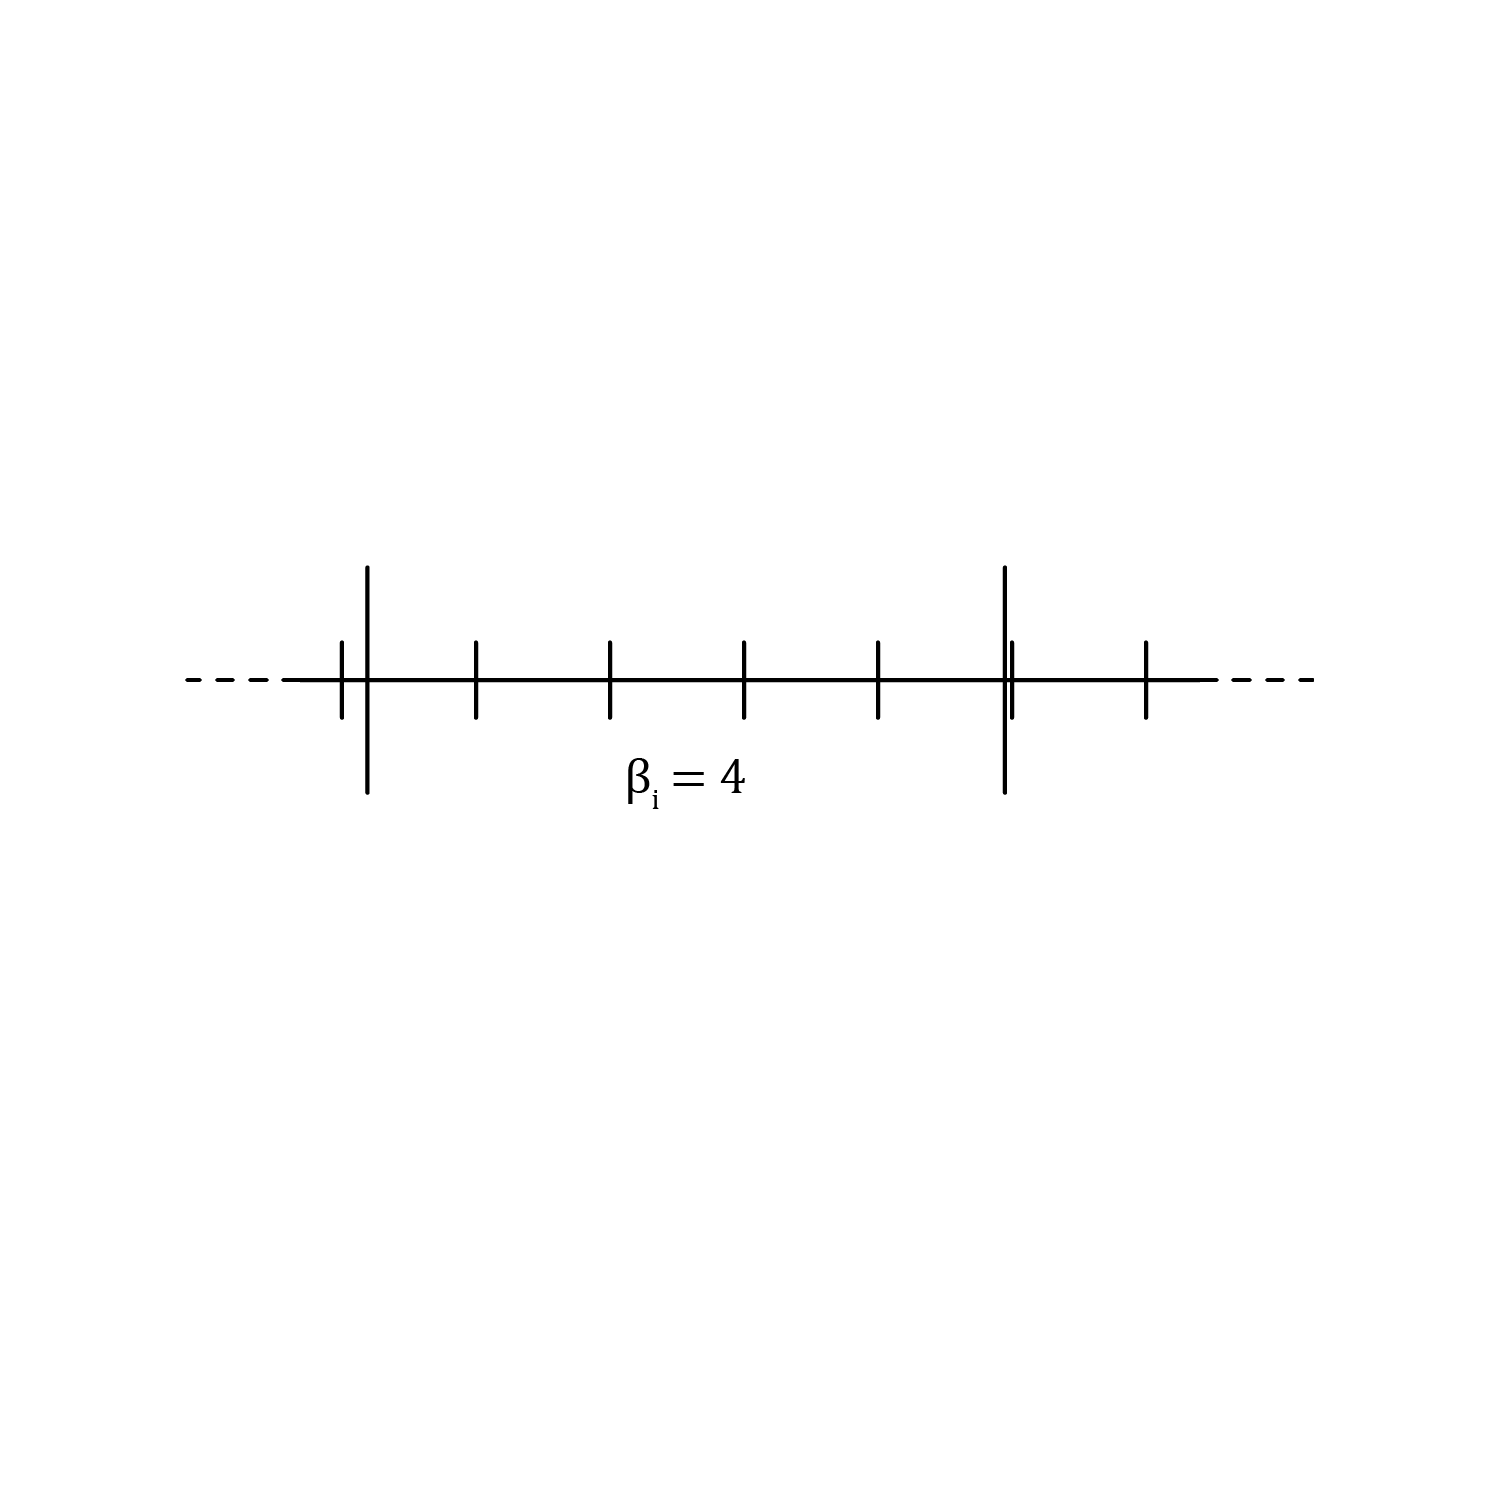
\includegraphics[width=3in]{sliding-window_2}
  \end{figure}
}

\frame{
	\frametitle{Windowing}
	\begin{figure}
    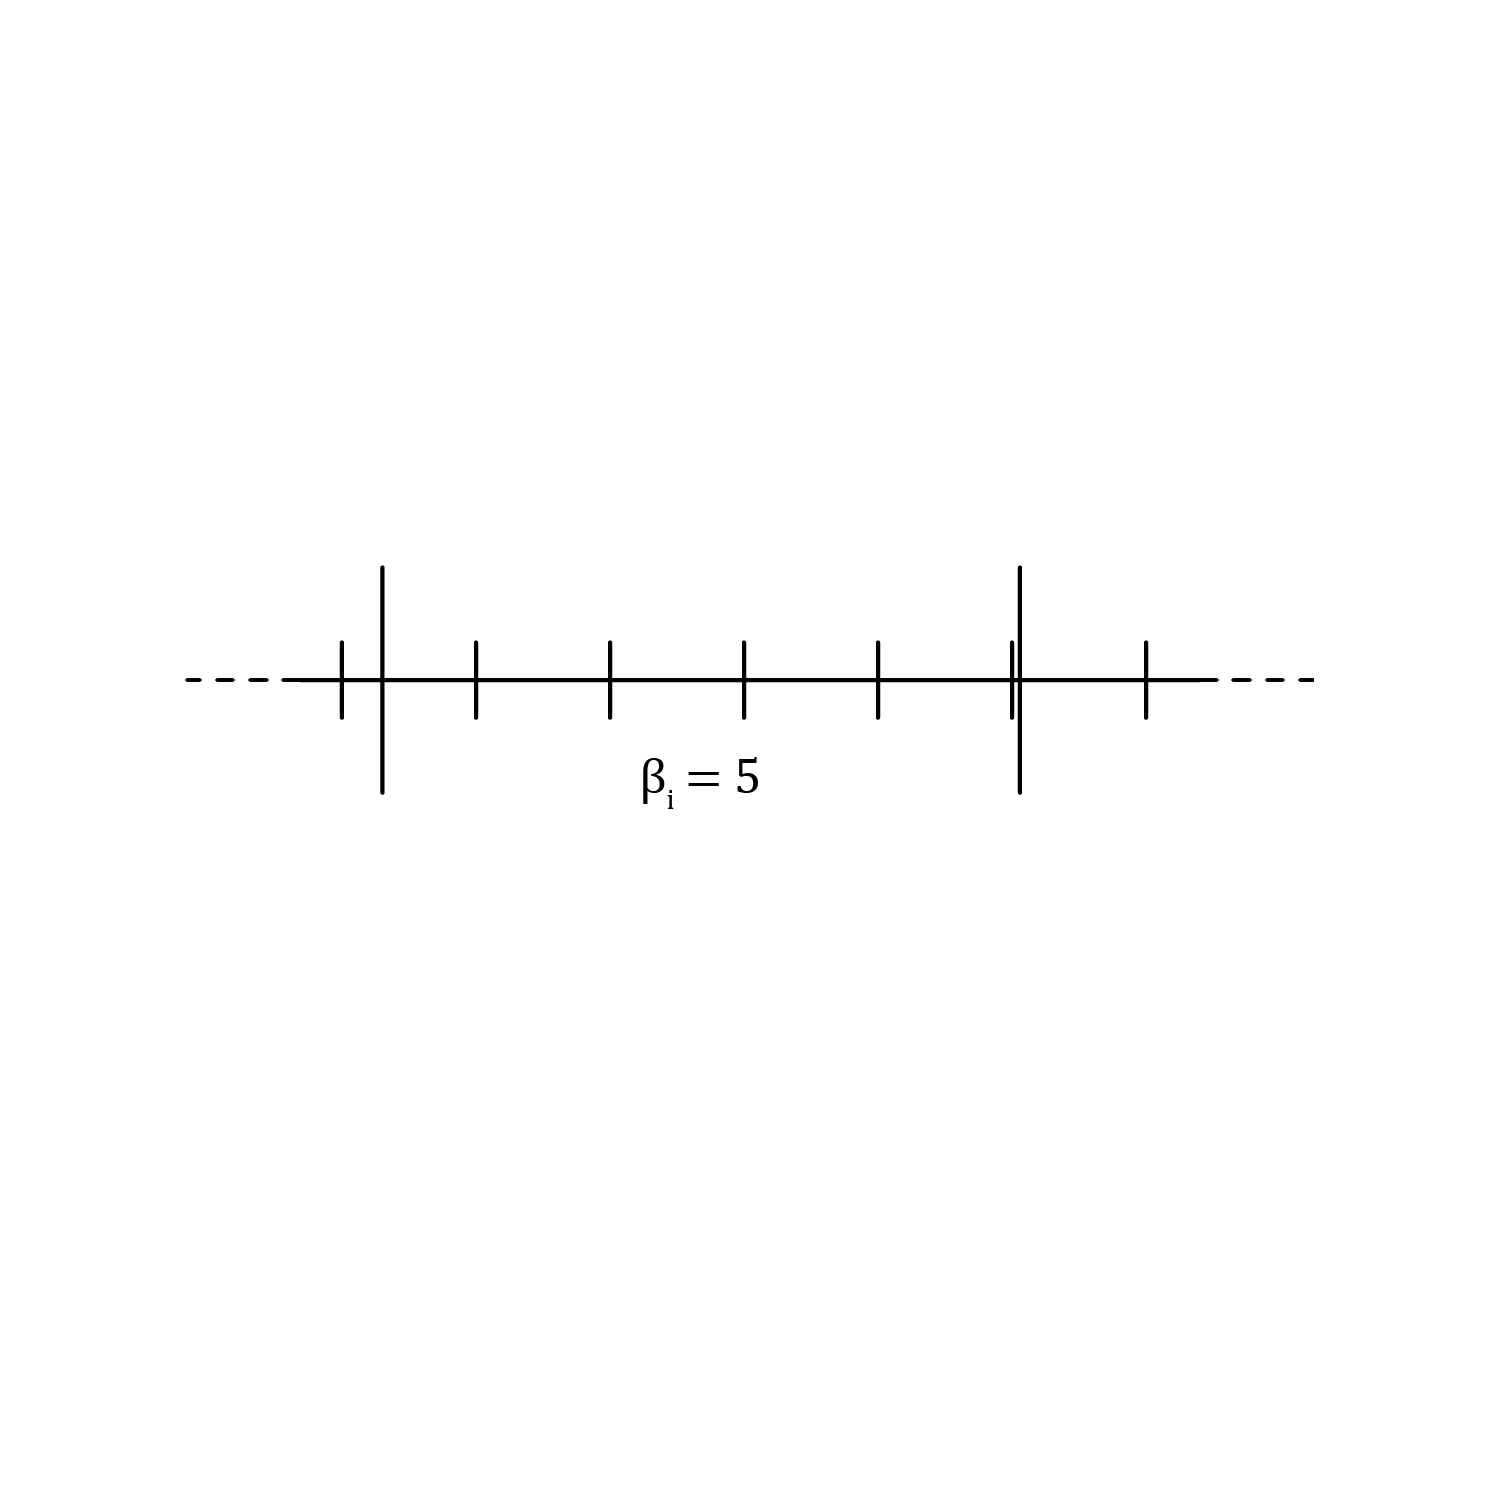
\includegraphics[width=3in]{sliding-window_3}
  \end{figure}
}

\frame{
	\frametitle{Windowing}
	\begin{figure}
    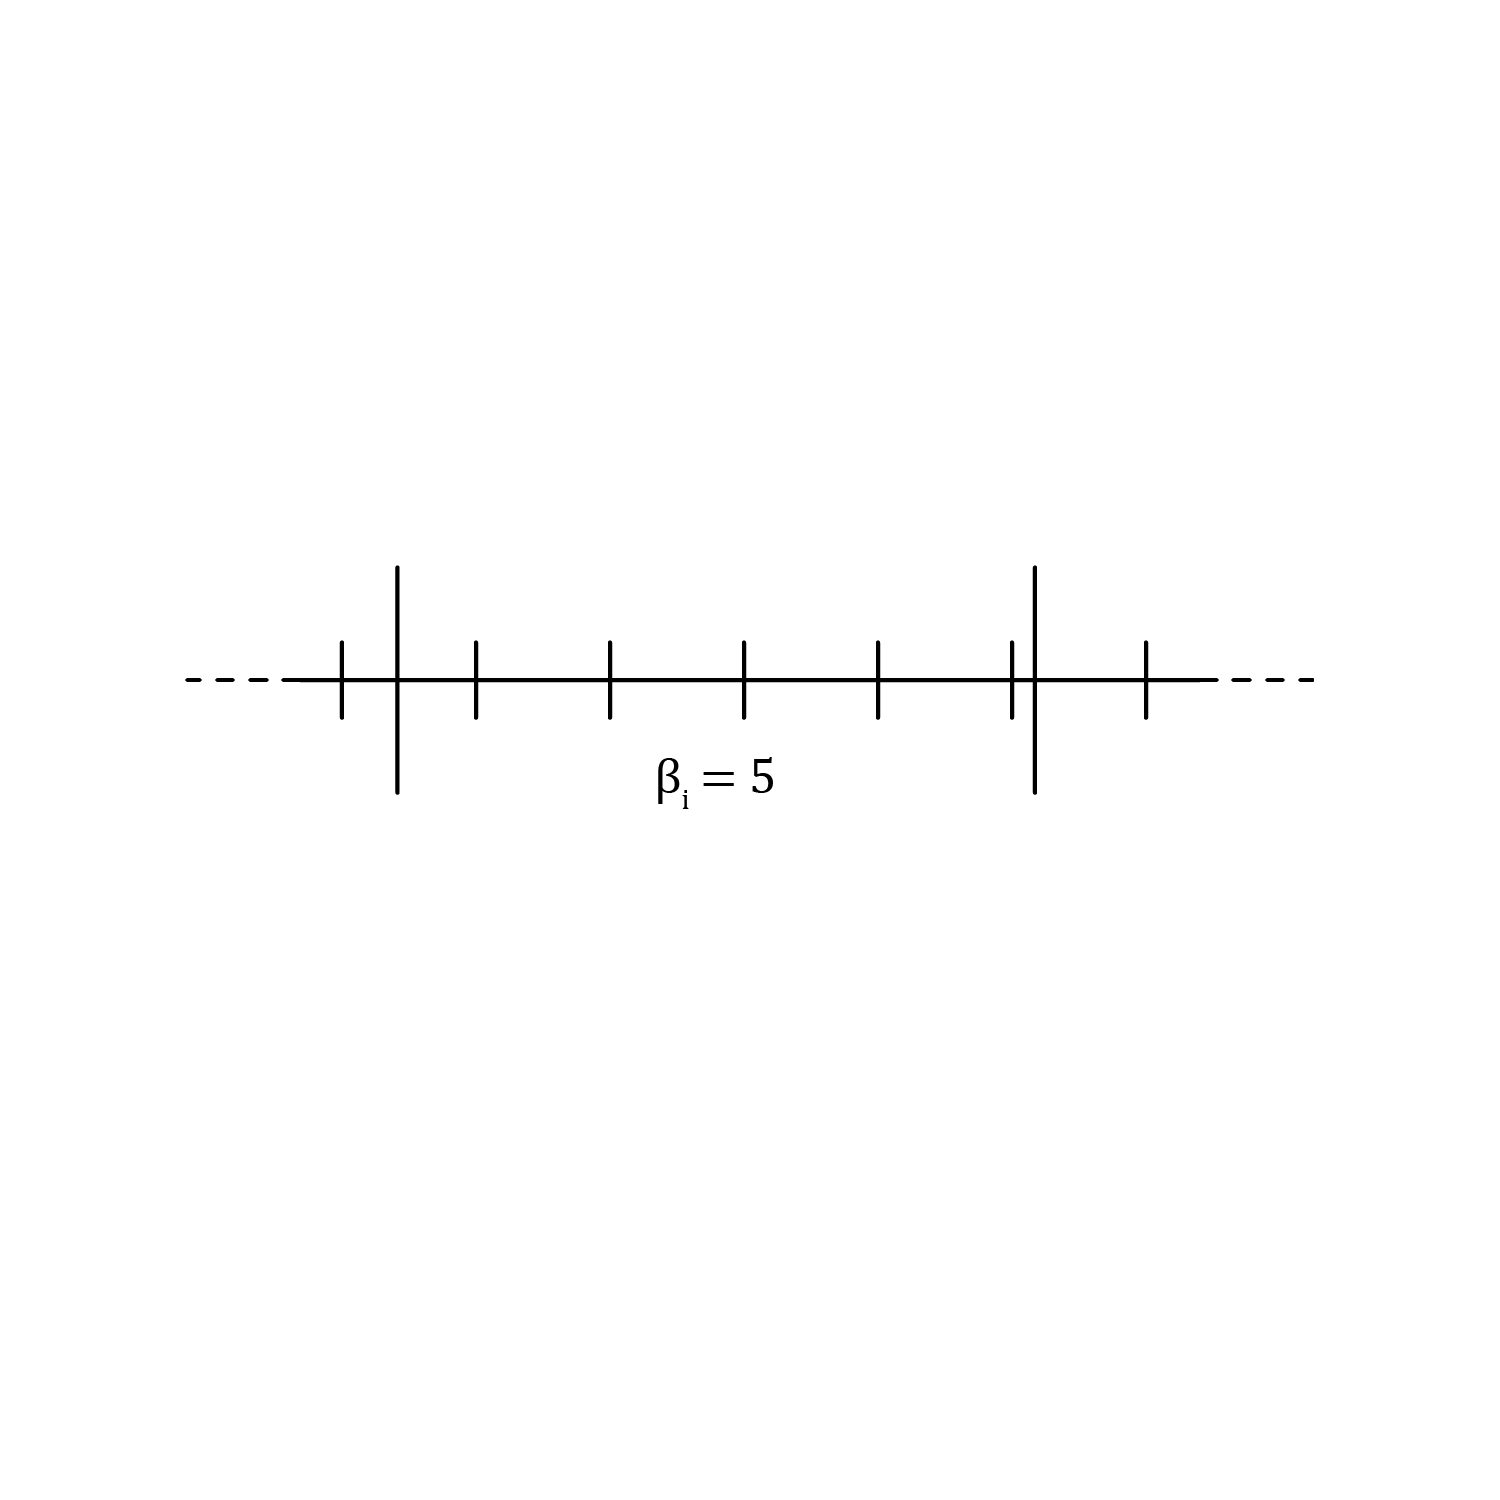
\includegraphics[width=3in]{sliding-window_4}
  \end{figure}
}

\frame{
	\frametitle{Windowing}
	\begin{figure}
    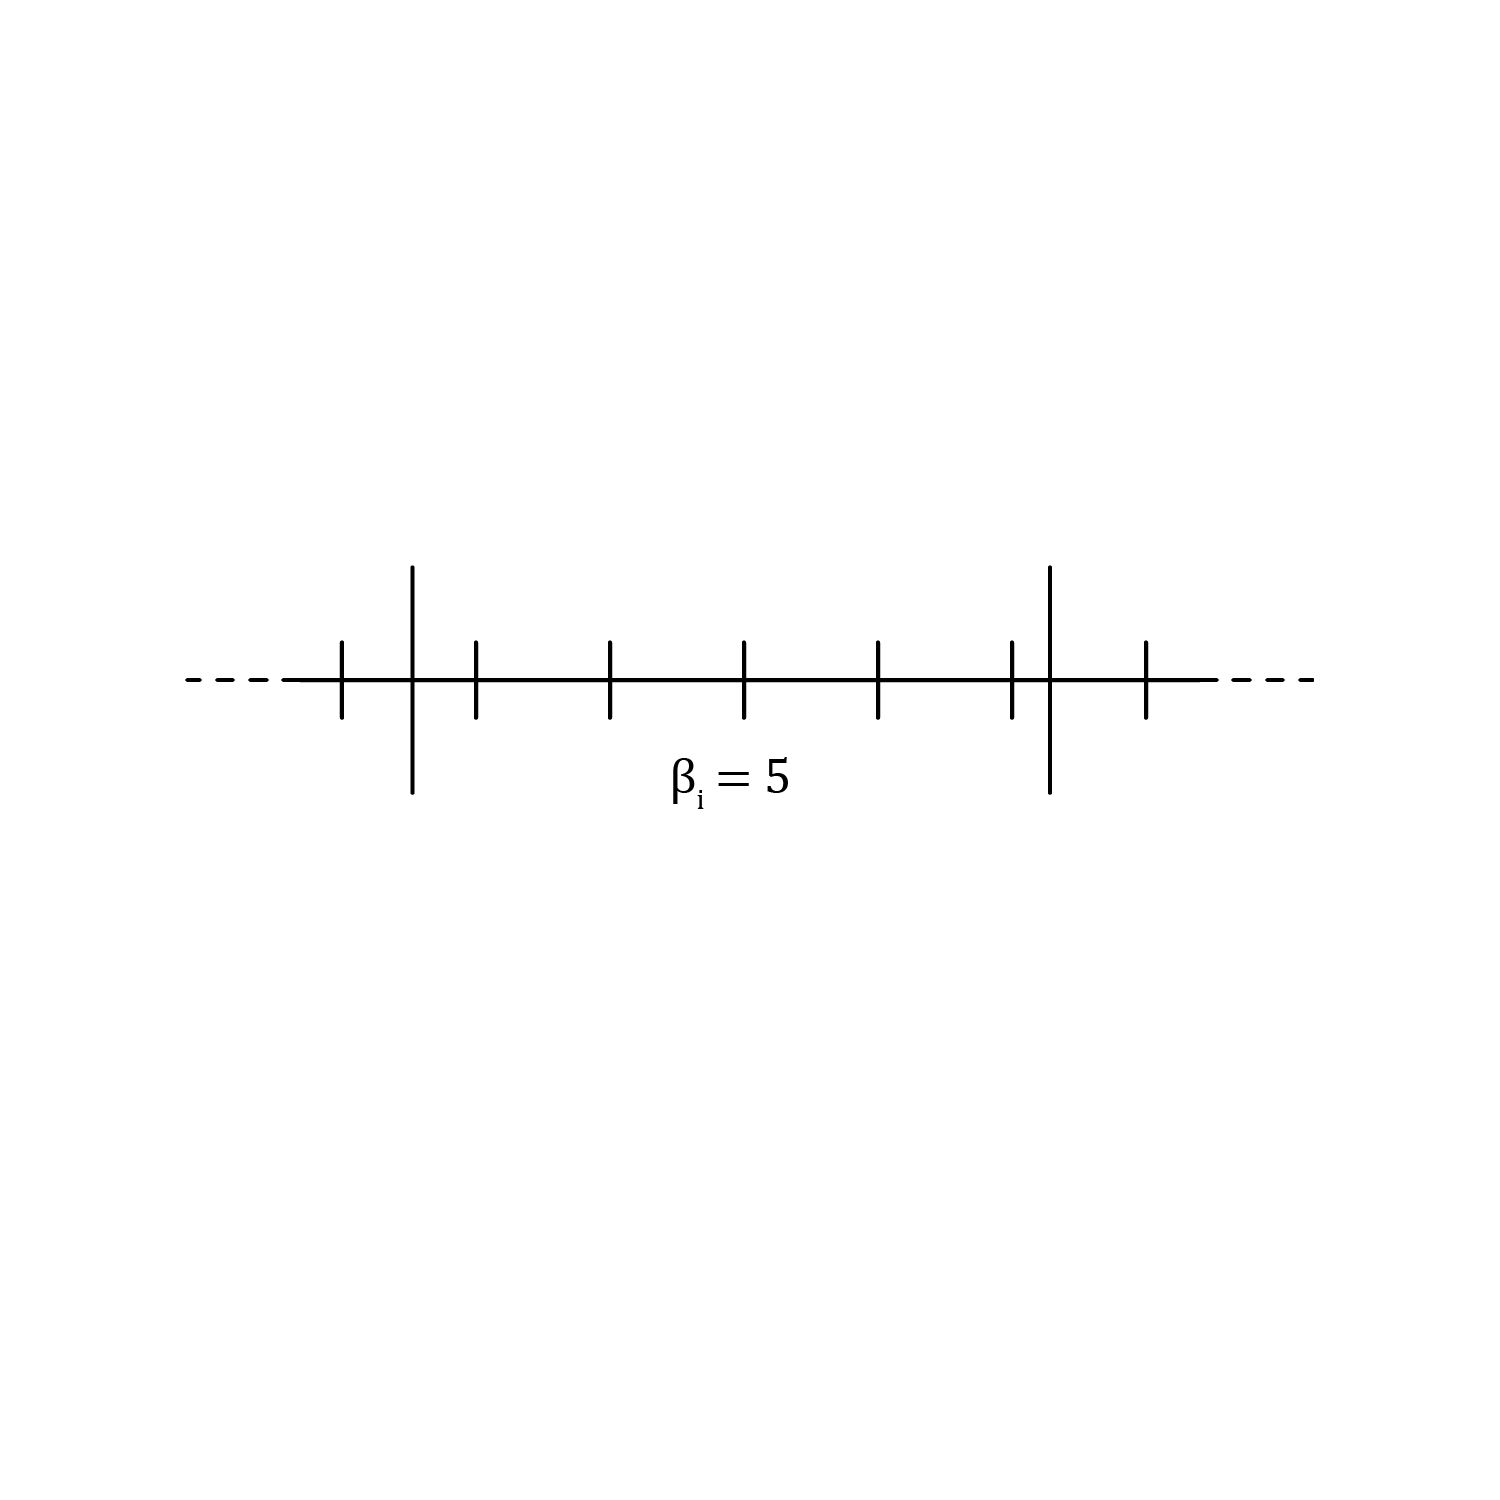
\includegraphics[width=3in]{sliding-window_5}
  \end{figure}
}

\frame{
	\frametitle{Windowing}
	\begin{figure}
    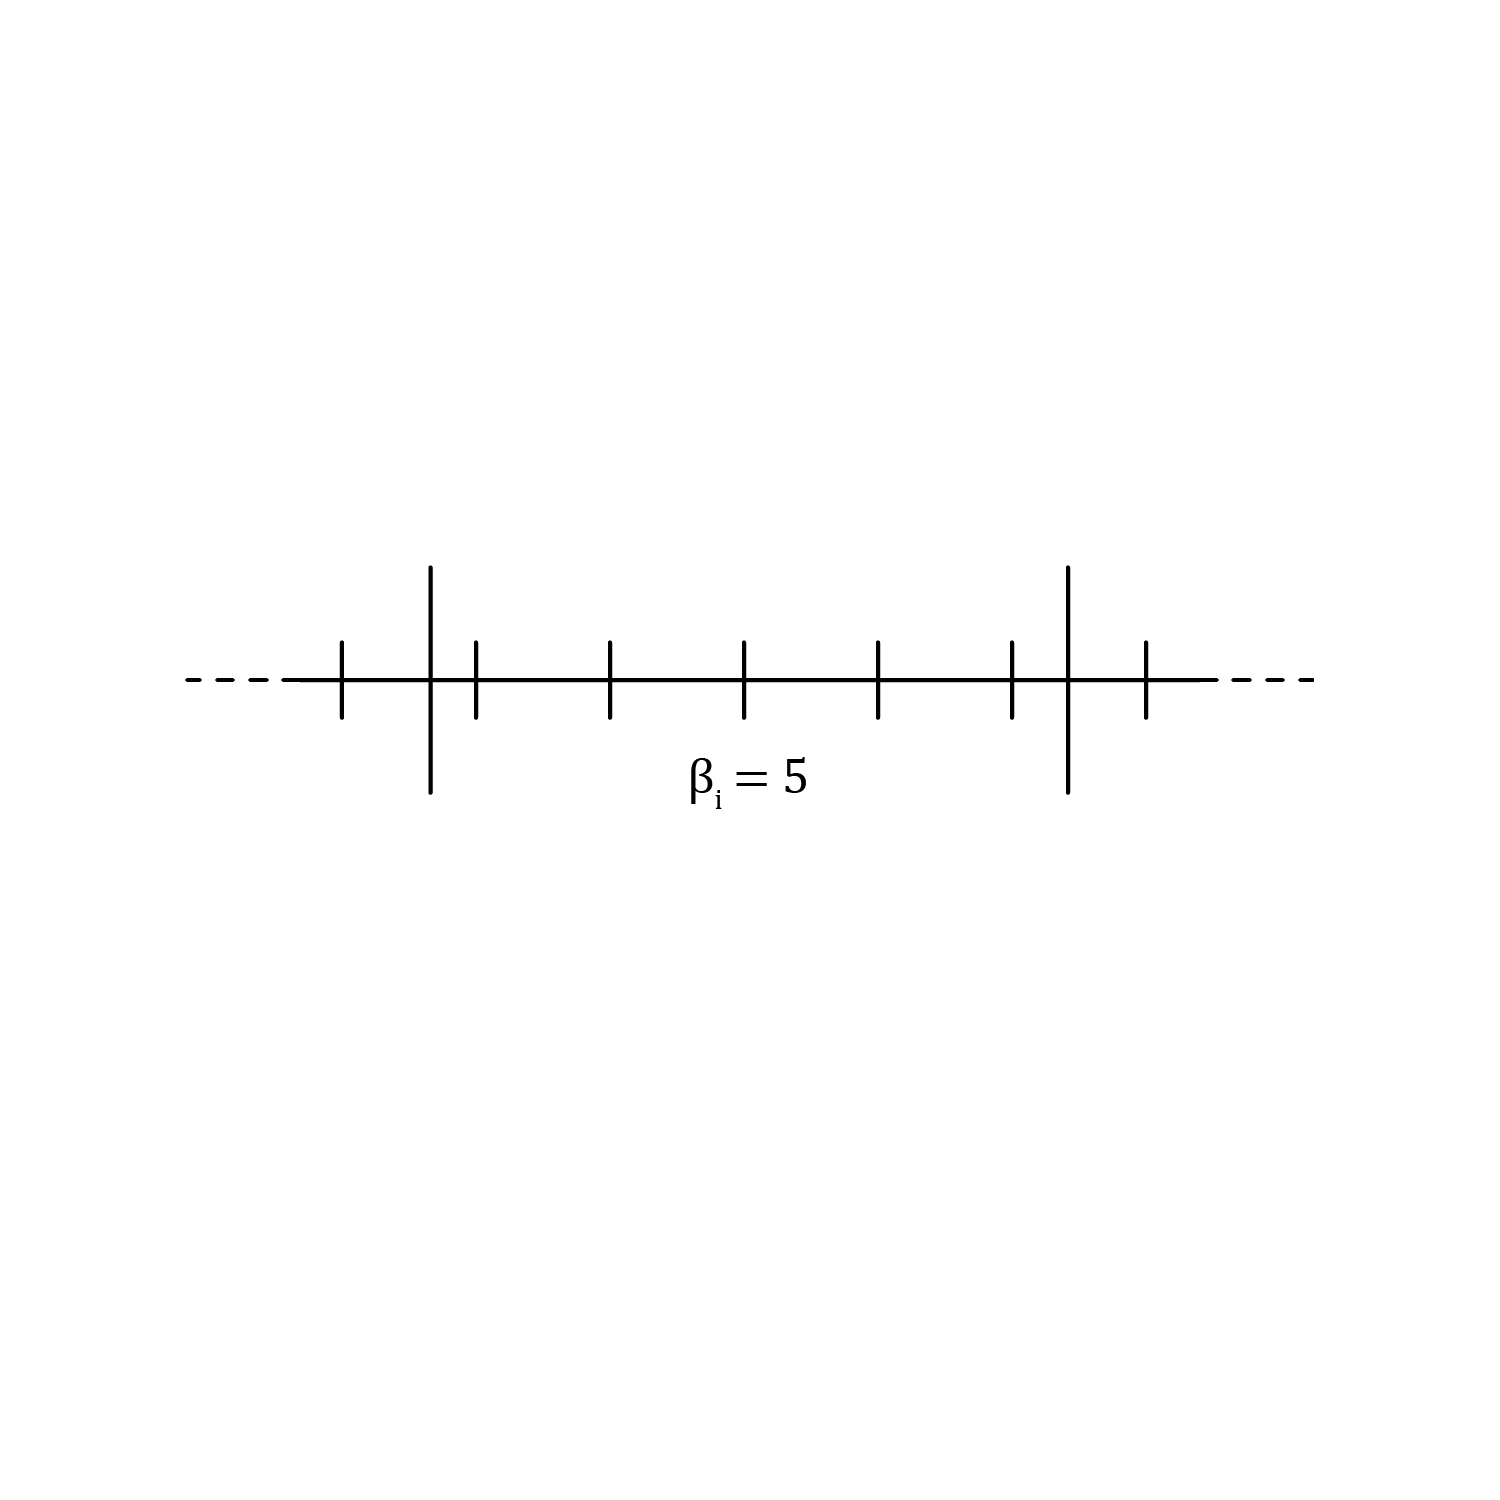
\includegraphics[width=3in]{sliding-window_6}
  \end{figure}
}

\frame{
	\frametitle{Windowing}
	\begin{figure}
    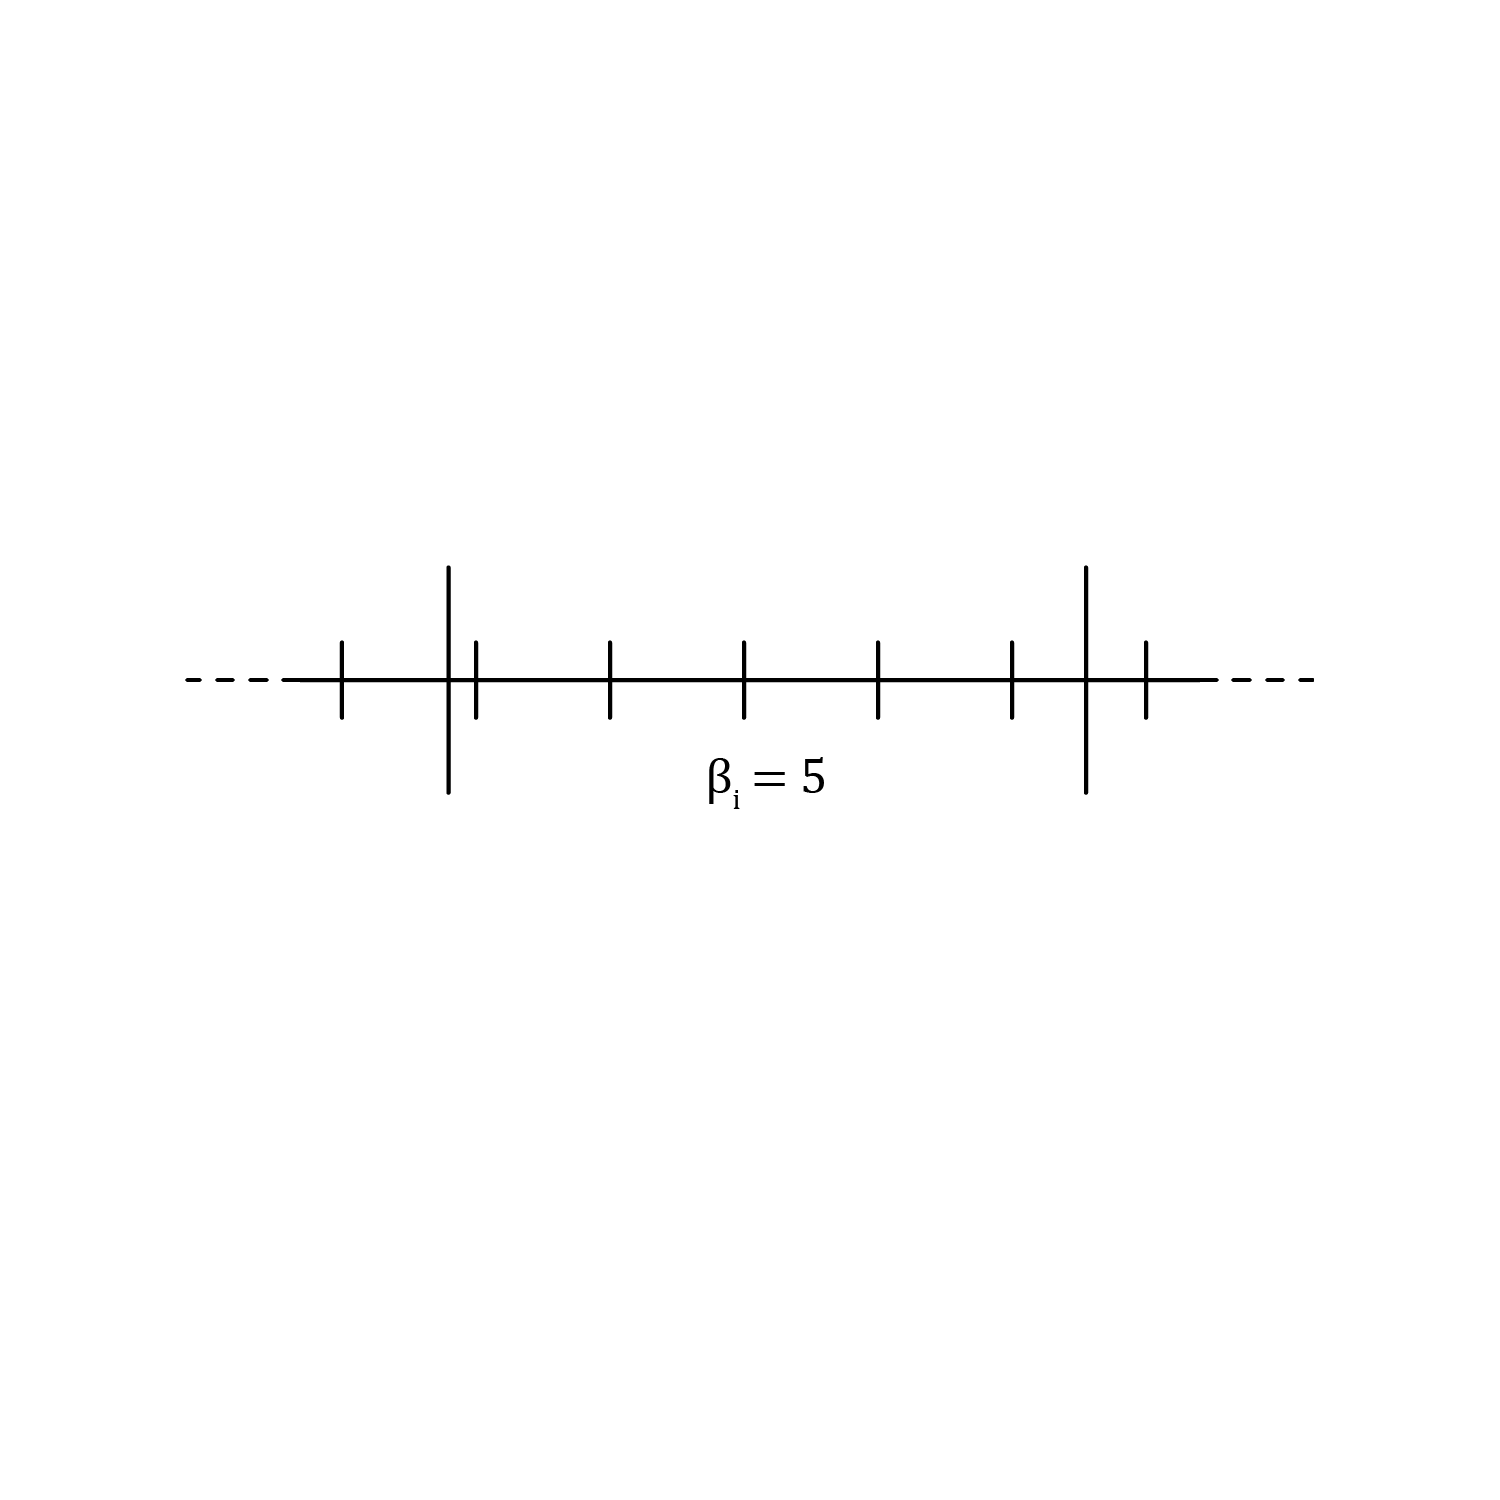
\includegraphics[width=3in]{sliding-window_7}
  \end{figure}
}

\frame{
	\frametitle{Windowing}
	\begin{figure}
    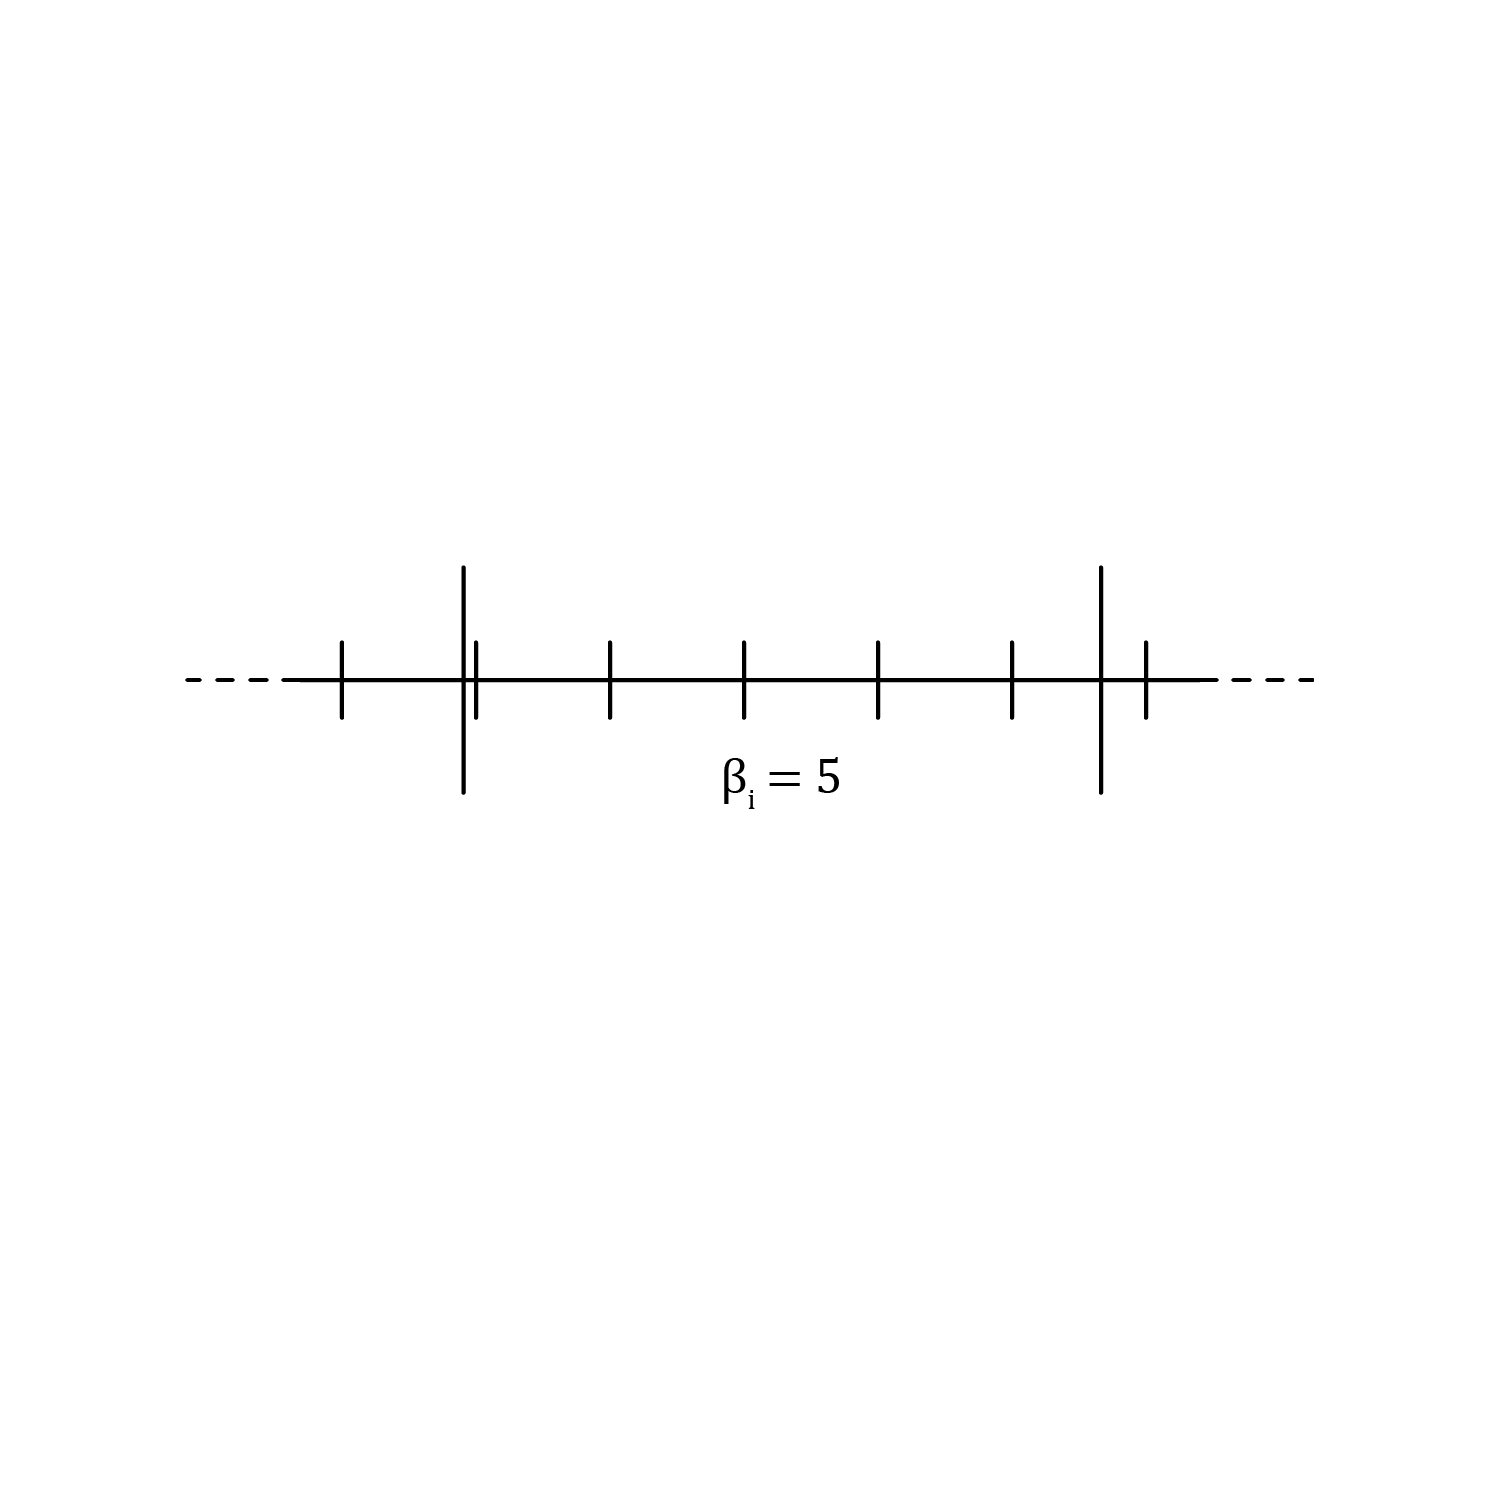
\includegraphics[width=3in]{sliding-window_8}
  \end{figure}
}

\frame{
	\frametitle{Windowing}
	\begin{figure}
    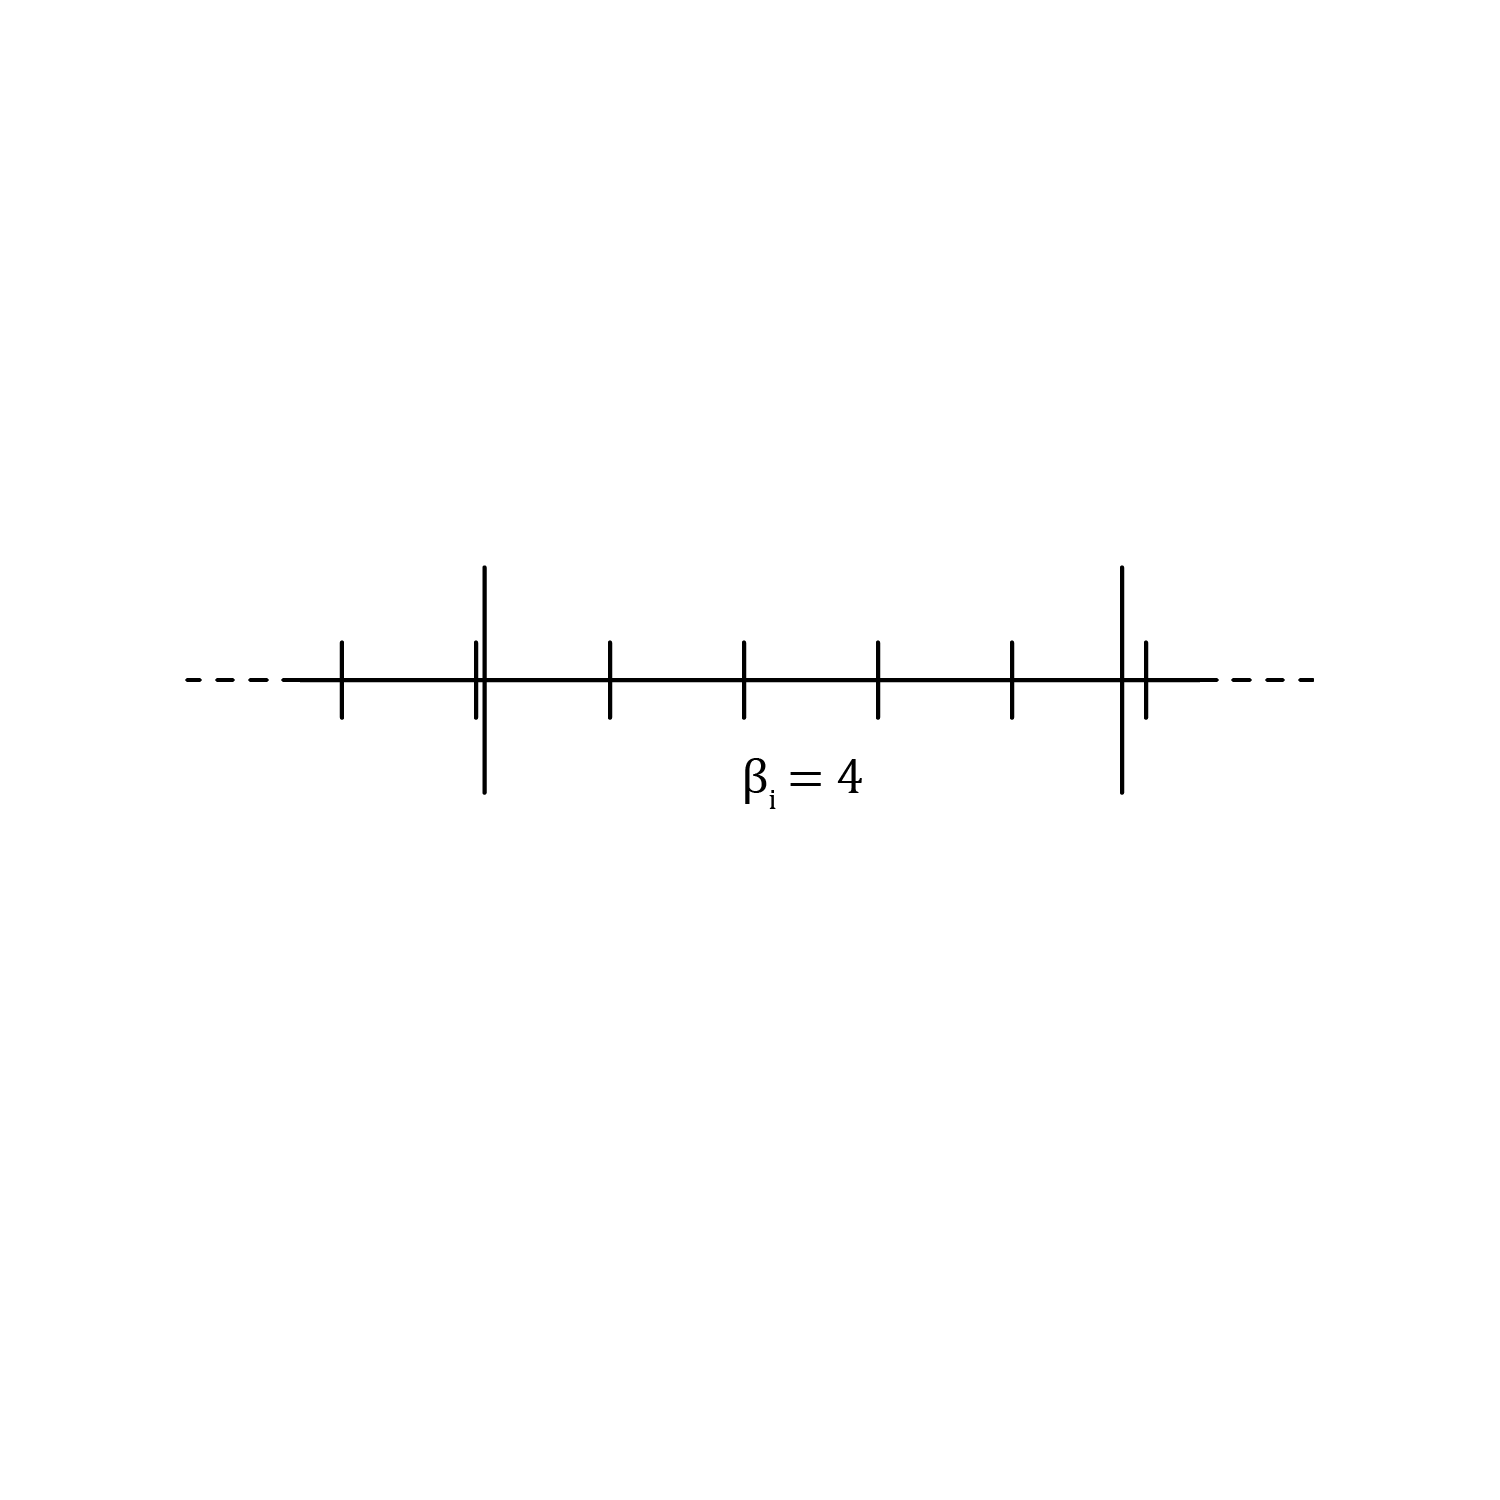
\includegraphics[width=3in]{sliding-window_9}
  \end{figure}
}

\frame{
	\frametitle{Windowing}
	\begin{figure}
    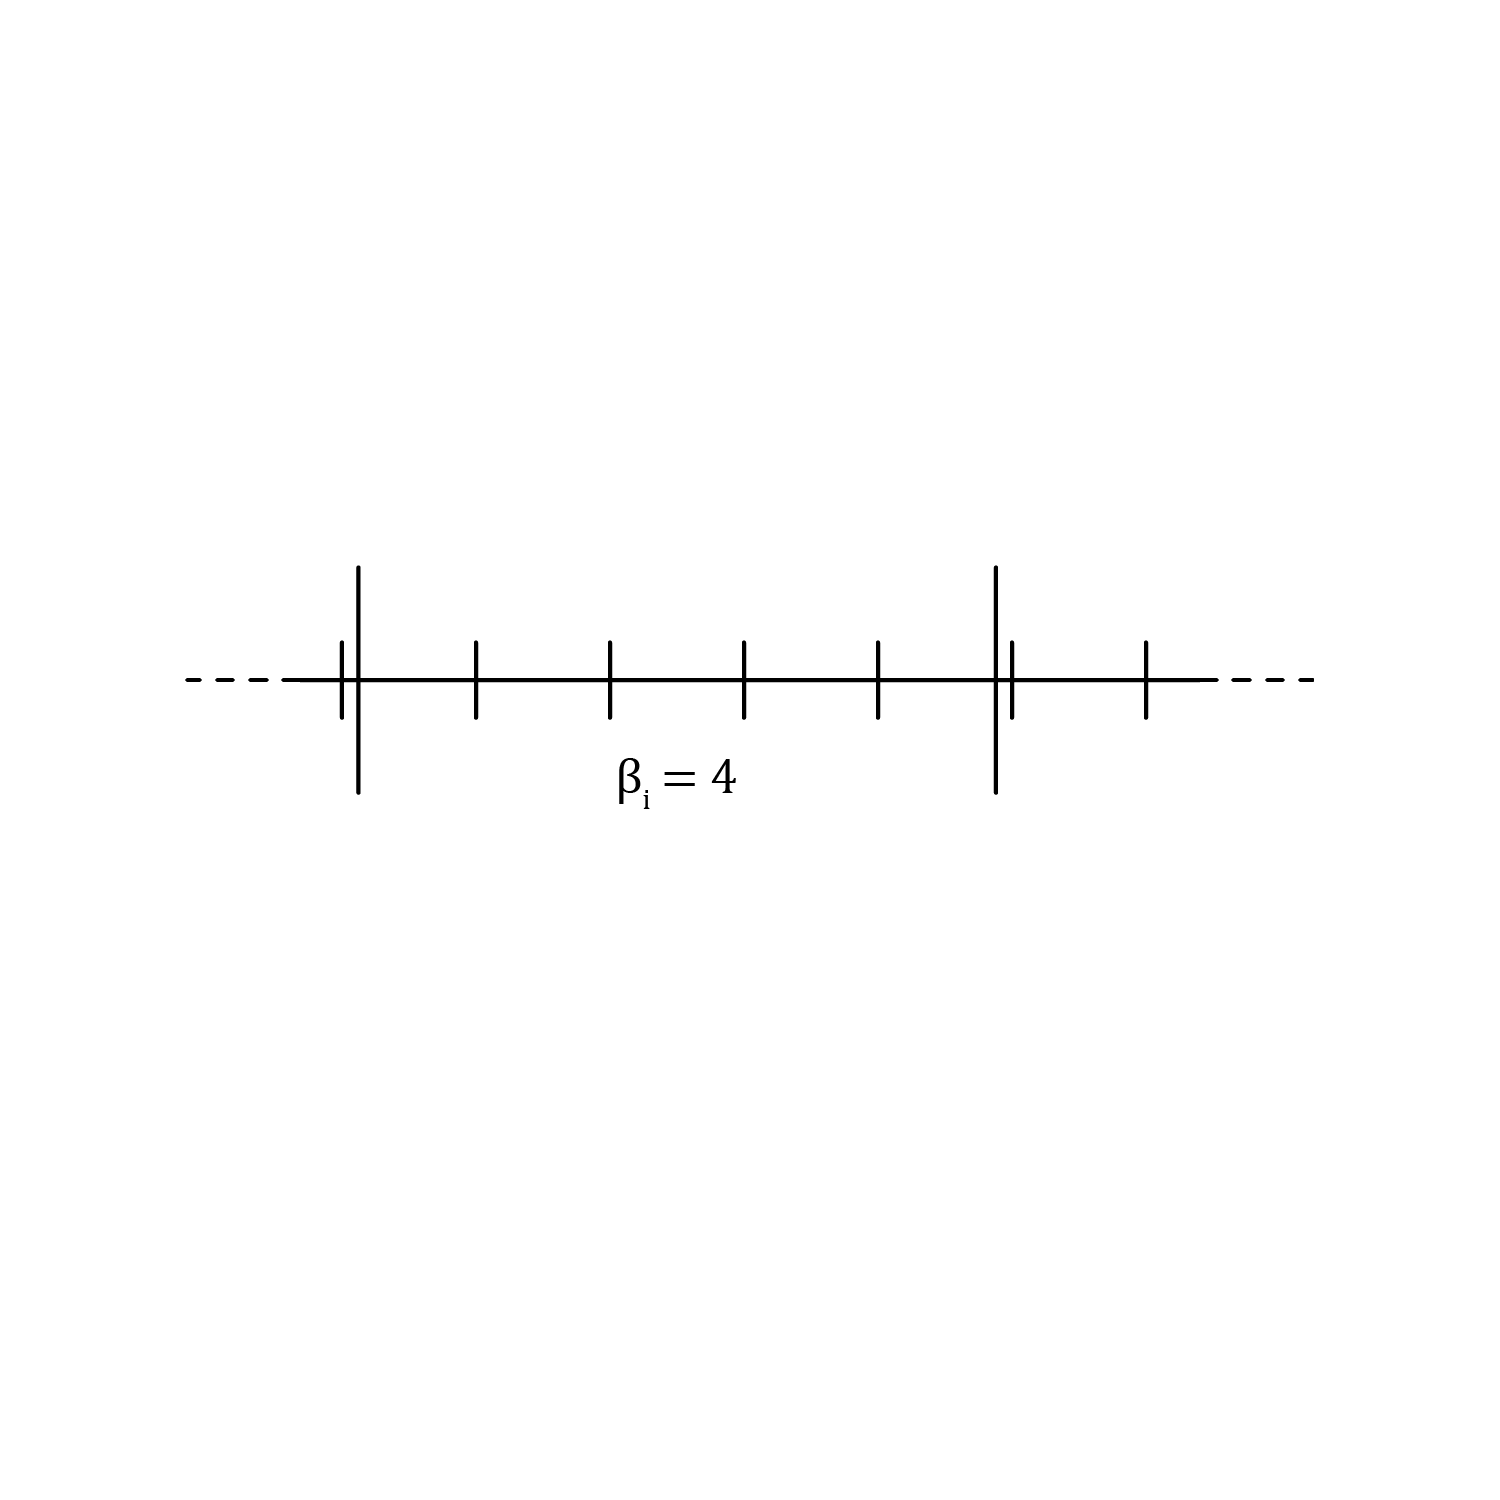
\includegraphics[width=3in]{sliding-window_1}
  \end{figure}
}